%-------------------------------------------------------------
%               FR CYBERDEF SECOPS BOOK
%              $File : coverback-book .tex
%                             2020 eduf@ction
%-------------------------------------------------------------
% 								BOOK FILES
%-------------------------------------------------------------

%----------------------------------------------------------------------------------------
%	4ième de COUVERTURE
%----------------------------------------------------------------------------------------
\pagestyle{empty}
\myemptypage

\newpage



\usetikzlibrary{shapes.geometric }
\usetikzlibrary{calc}

\colorlet{covercolor}{edxcolorcover}

\begin{tikzpicture}[remember picture,overlay]
%%%%%%%%%%%%%%%%%%%% Background %%%%%%%%%%%%%%%%%%%%%%%%
\fill[covercolor] (current page.south west) rectangle (current page.north east);


\foreach \i in {2.5,...,22}
{
    \node[rounded corners,covercolor!60,draw,regular polygon,regular polygon sides=6, minimum size=\i cm,ultra thick] at ($(current page.west)+(2.5,-5)$) {} ;
}

%%%%%%%%%%%%%%%%%%%% Background Polygon %%%%%%%%%%%%%%%%%%%% 
\foreach \i in {0.5,...,22}
{
\node[rounded corners,covercolor!60,draw,regular polygon,regular polygon sides=6, minimum size=\i cm,ultra thick] at ($(current page.north west)+(2.5,0)$) {} ;
}

\foreach \i in {0.5,...,22}
{
\node[rounded corners,covercolor!90,draw,regular polygon,regular polygon sides=6, minimum size=\i cm,ultra thick] at ($(current page.north east)+(0,-9.5)$) {} ;
}


\foreach \i in {21,...,6}
{
\node[covercolor!85,rounded corners,draw,regular polygon,regular polygon sides=6, minimum size=\i cm,ultra thick] at ($(current page.south east)+(-0.2,-0.45)$) {} ;
}


\draw (current page.north west) node [fill=ocre!00!white,fill opacity=0,text opacity=1,inner sep=0cm,xshift= 6 cm,  yshift=-17 cm, anchor=north west]
{\centering\sffamily\parbox[c][][t]{13cm}{\small \color{white} Eric DUPUIS (Enseignant SEC101, Cnam Bretagne) est actuellement Directeur d'Orange Campus Cyber, le centre de formation et d'entrainement Cybersécurité et Cyberdéfense du groupe Orange après plusieurs années comme directeur sécurité de la société Orange Cyberdefense. Ingénieur des corps techniques de l’armement du ministère des armées, il a exercé pendant plusieurs années à la Délégation Générale pour l’Armement  / Maitrise de l'information (DGA/MI) dans les domaines du renseignement, de la lutte informatique et de la cyberdéfense.\\
Ingénieur du Conservatoire National des Art et Métiers, il y enseigne l’ingénierie et la sécurité du numérique.  Auditeur de la 50ième session Armement et Economie de Défense de l’IHEDN (Institut des Hautes Etudes de la Défense National), il intervient au profit de la Gendarmerie, en tant qu'Officier de Réserve Cyberdéfense.
\\}};
% ------Descriptif de l'ouvrage--------------------------------------------------------------------------------------
\draw (current page.north west) node [fill=ocre!00!white,fill opacity=1,text opacity=1,inner sep=1cm,xshift= 2 cm,  yshift=-4 cm, anchor=north west]
{\centering\sffamily\parbox[c][][t]{15cm}{\normalsize Aborder la sécurité des systèmes d’information sous l’angle d'une sécurité dynamique est un axe qui depuis quelques années apporte de nouvelle manière d’aborder la protection, la défense, et la résilience des systèmes d’information. La transformation digitale de l'entreprise modifie et rend plus flous les périmètres des systèmes d’informations. Cela nécessite une approche élargie du risque numérique et des nouvelles architectures de cybersécurité. Malgré la mise en place de mesures et de technologies de protection de plus en plus élaborées, l'impact d'une attaque ayant franchi ces barrières à considérablement augmenté.  Cette compilation des notes de cours élaborée dans le cadre d'un cours d'introduction à la gouvernance de la cybersécurité aborde une démarche de cyberdéfense d’entreprise construite à partir de quelques éléments fondamentaux. Protéger l'ensemble de l'entreprise alors qu'il est complexe de définir ses frontières est illusoire. Identifier les actifs essentiels ou vitaux et mettre en place les moyens adaptés à leur protection et leur défense est une démarche tactique qui permet de graduellement réduire ses cyber-risques.  Issu de ce cours sur le déploiement de politiques de cyberdéfense, cet ouvrage décrit quelques éléments essentiels de sécurité opérationnelle permettant de fixer, à partir d’une analyse des risques, des priorités opérationnelles tant sur l'organisation des processus que des architectures de protection, de défense et de résilience.}};

% ------PHOTO--------------------------------------------------------------------------------------
\node at (current page.north west)   [xshift= 2cm,  yshift=-17cm, anchor=north west]  {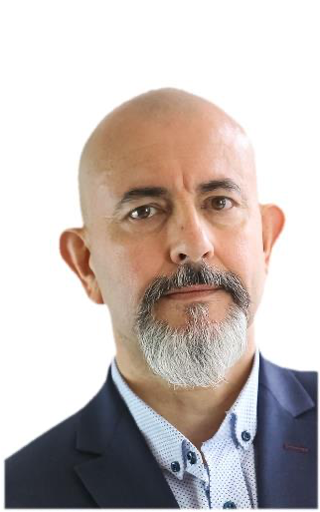
\includegraphics[width=3cm]{\upath/template.inc/CourseModel/CoursePictures/edu.png}}; 


% ------EAN--------------------------------------------------------------------------------------
%\node at (current page.north west)   [xshift= 15cm,  yshift=-24cm, anchor=north west]  {
\includegraphics[width=4cm]{\upath/template.inc/BookModel/BookPictures/ean-white.pdf} }; 

% ------TITRE DE BAS DE PAGE --------------------------------------------------------------------------------------
\node at (current page.center)  [xshift=0cm, yshift=-11cm, text opacity=1]  { {\centering \huge\color{white}\bfseries\sffamily \ubooktitleMain} } ; 

\node at (current page.center)  [xshift=0cm, yshift=-12cm, text opacity=1]  {{\centering \huge\color{white}\bfseries\sffamily \ccbyncndeu}  } ; 



%%%%%%%%%%%%%%%%%%%%% Title of the Report %%%%%%%%%%%%%%%%%%%% 
%\node[left,covercolor!5,minimum width=0.625*\paperwidth,minimum height=3cm, rounded corners] at ($(current page.north east)+(0,-9.5)$)
%{
%{\fontsize{40}{30} \selectfont \bfseries CYBERDEF 101}
%};
%
%%%%%%%%%%%%%%%%%%%%% Subtitle %%%%%%%%%%%%%%%%%%%% 
%\node[left,covercolor!10,minimum width=0.625*\paperwidth,minimum height=2cm, rounded corners] at ($(current page.north east)+(0,-11)$)
%{
%{\huge \textit{Sécurité Opérationelle}}
%};
%
%%%%%%%%%%%%%%%%%%%%% Author Name %%%%%%%%%%%%%%%%%%%% 
%\node[left,covercolor!5,minimum width=0.625*\paperwidth,minimum height=2cm, rounded corners] at ($(current page.north east)+(0,-13)$)
%{
%{\Large \textsc{Eric DUPUIS}}
%};

%%%%%%%%%%%%%%%%%%%% Year %%%%%%%%%%%%%%%%%%%% 
%\node[rounded corners,fill=covercolor!80,text =covercolor!5,regular polygon,regular polygon sides=6, minimum size=2.5 cm,inner sep=0,ultra thick] at ($(current page.west)+(2.5,-5)$) {\LARGE \bfseries 2023};
%
%\node at ($(current page.north east)+(0,-13)$)[xshift=-4cm, yshift=-11cm]  { 
\includegraphics[width=0.2\paperwidth]{\upath/template.inc/BookModel/BookPictures/shield-20-white.pdf}} ;
%
%
%\node at (current page.center)  [xshift=0cm, yshift=13 cm, text opacity=1]  { {\color{white}\printer} } ; 




\end{tikzpicture}


